\documentclass{article}
%\documentclass[pra,aps]{revtex4}
\usepackage{natbib} 
\usepackage{graphics} % use the graphics package for simple commands
\usepackage{graphicx} % or use the graphicx package for more complicated commands
\usepackage{epsfig} % or use epsfig package if you prefer to use the old commands
\usepackage{amssymb} % The amssymb package provides various useful mathematical symbols
\usepackage{amsmath}

\newcommand{\ket}[1]{\ensuremath{\left| #1 \right\rangle}}
\newcommand{\bra}[1]{\ensuremath{\left\langle #1 \right|}}
\newcommand{\braket}[2]{\ensuremath{\left\langle #1 \right|\left. #2 \right\rangle}}
\newcommand{\expect}[1]{\ensuremath{\left\langle #1 \right\rangle}}
\newcommand{\eV}{\mbox{eV}}
\newcommand{\icm}{\ensuremath{\mbox{cm}^{-1}}}
\newcommand{\cm}{\mbox{cm}}
\newcommand{\EE}[1]{\ensuremath{\times 10^{ #1 }}}
\newcommand{\ee}[1]{\ensuremath{\times 10^{ #1 }}}
\newcommand{\norm}[1]{\ensuremath{\left| #1 \right|}}
\newcommand{\abs}[1]{\ensuremath{\left| #1 \right|}}
\newcommand{\HH}{\mathcal{H}}
\newcommand{\laplace}[1]{\ensuremath{\mathcal{L}\left\{ #1 \right\}}}
\newcommand{\fourier}[1]{\ensuremath{\mathcal{F}\left\{ #1 \right\}}}
\newcommand{\invlaplace}[1]{\ensuremath{\mathcal{L}^{-1}\left\{ #1 \right\}}}
\newcommand{\invfourier}[1]{\ensuremath{\mathcal{F}^{-1}\left\{ #1 \right\}}}
\newcommand{\myexp}[1]{\ensuremath{ \exp\left( #1 \right) }}
\newcommand{\eps}{\varepsilon}
\newcommand{\myerf}[1]{\ensuremath{{\mathrm{erf}\left( #1 \right)}}}
\newcommand{\heaviside}[1]{\ensuremath{ \mathrm{\Theta}\left( #1 \right)}}
\newcommand{\etal}{,~\textit{et~al.,~}}

\graphicspath{{../figs/}}
\newlength{\figwidth}
\setlength{\figwidth}{.9\linewidth}

\begin{document}

\author{Ryan Coffee, Nick Hartmann, Andreas Galler, Markus Ilchen
, Timur Y Osipov
, more\ldots}
%\affiliation{SLAC National Accelerator laboratory, Menlo Park, California, USA}
%\affiliation{The PULSE Institute, Stanford, California, USA}
%\affiliation{European XFEL, Hamburg, Germany}

\title{Time-shear interference for x-ray/optical cross-correlation timing at high repetition rate x-ray free-electron lasers.}

\begin{abstract}
In this report, we present results that demonstrate orders of magnitude improvement in signal sensitivity for x-ray optical cross correlation as used for relative delay identification.
For both so called ``warm'' accelerator based x-ray Free Electron Lasers (xFELs) and the new superconducting quasi-continous high repetition rate xFELs, there still is a need for shot-by-shot arrival time measurement and sorting.
\end{abstract}

\maketitle


\section{Introduction}
\subsection{Jitter}
State the existing problem
\subsubsection{History}
State the old way of fixing it
\subsubsection{Stochastic sampling paradigm}
\subsubsection{Expectations at EuXFEL and LCLS-II}
\subsection{Diamond}
\subsubsection{Thermal Load}
	But with the higher repetition rate xFELs, the average power load on x-ray optics is so high that we need extremely highly conducing cross correlation medium.
\subsubsection{Absorption}
	sensitivity
\subsubsection{Historical trials}

\subsection{Time-shear interference}
State the new interference

\section{Method}
\begin{figure}
\centerline{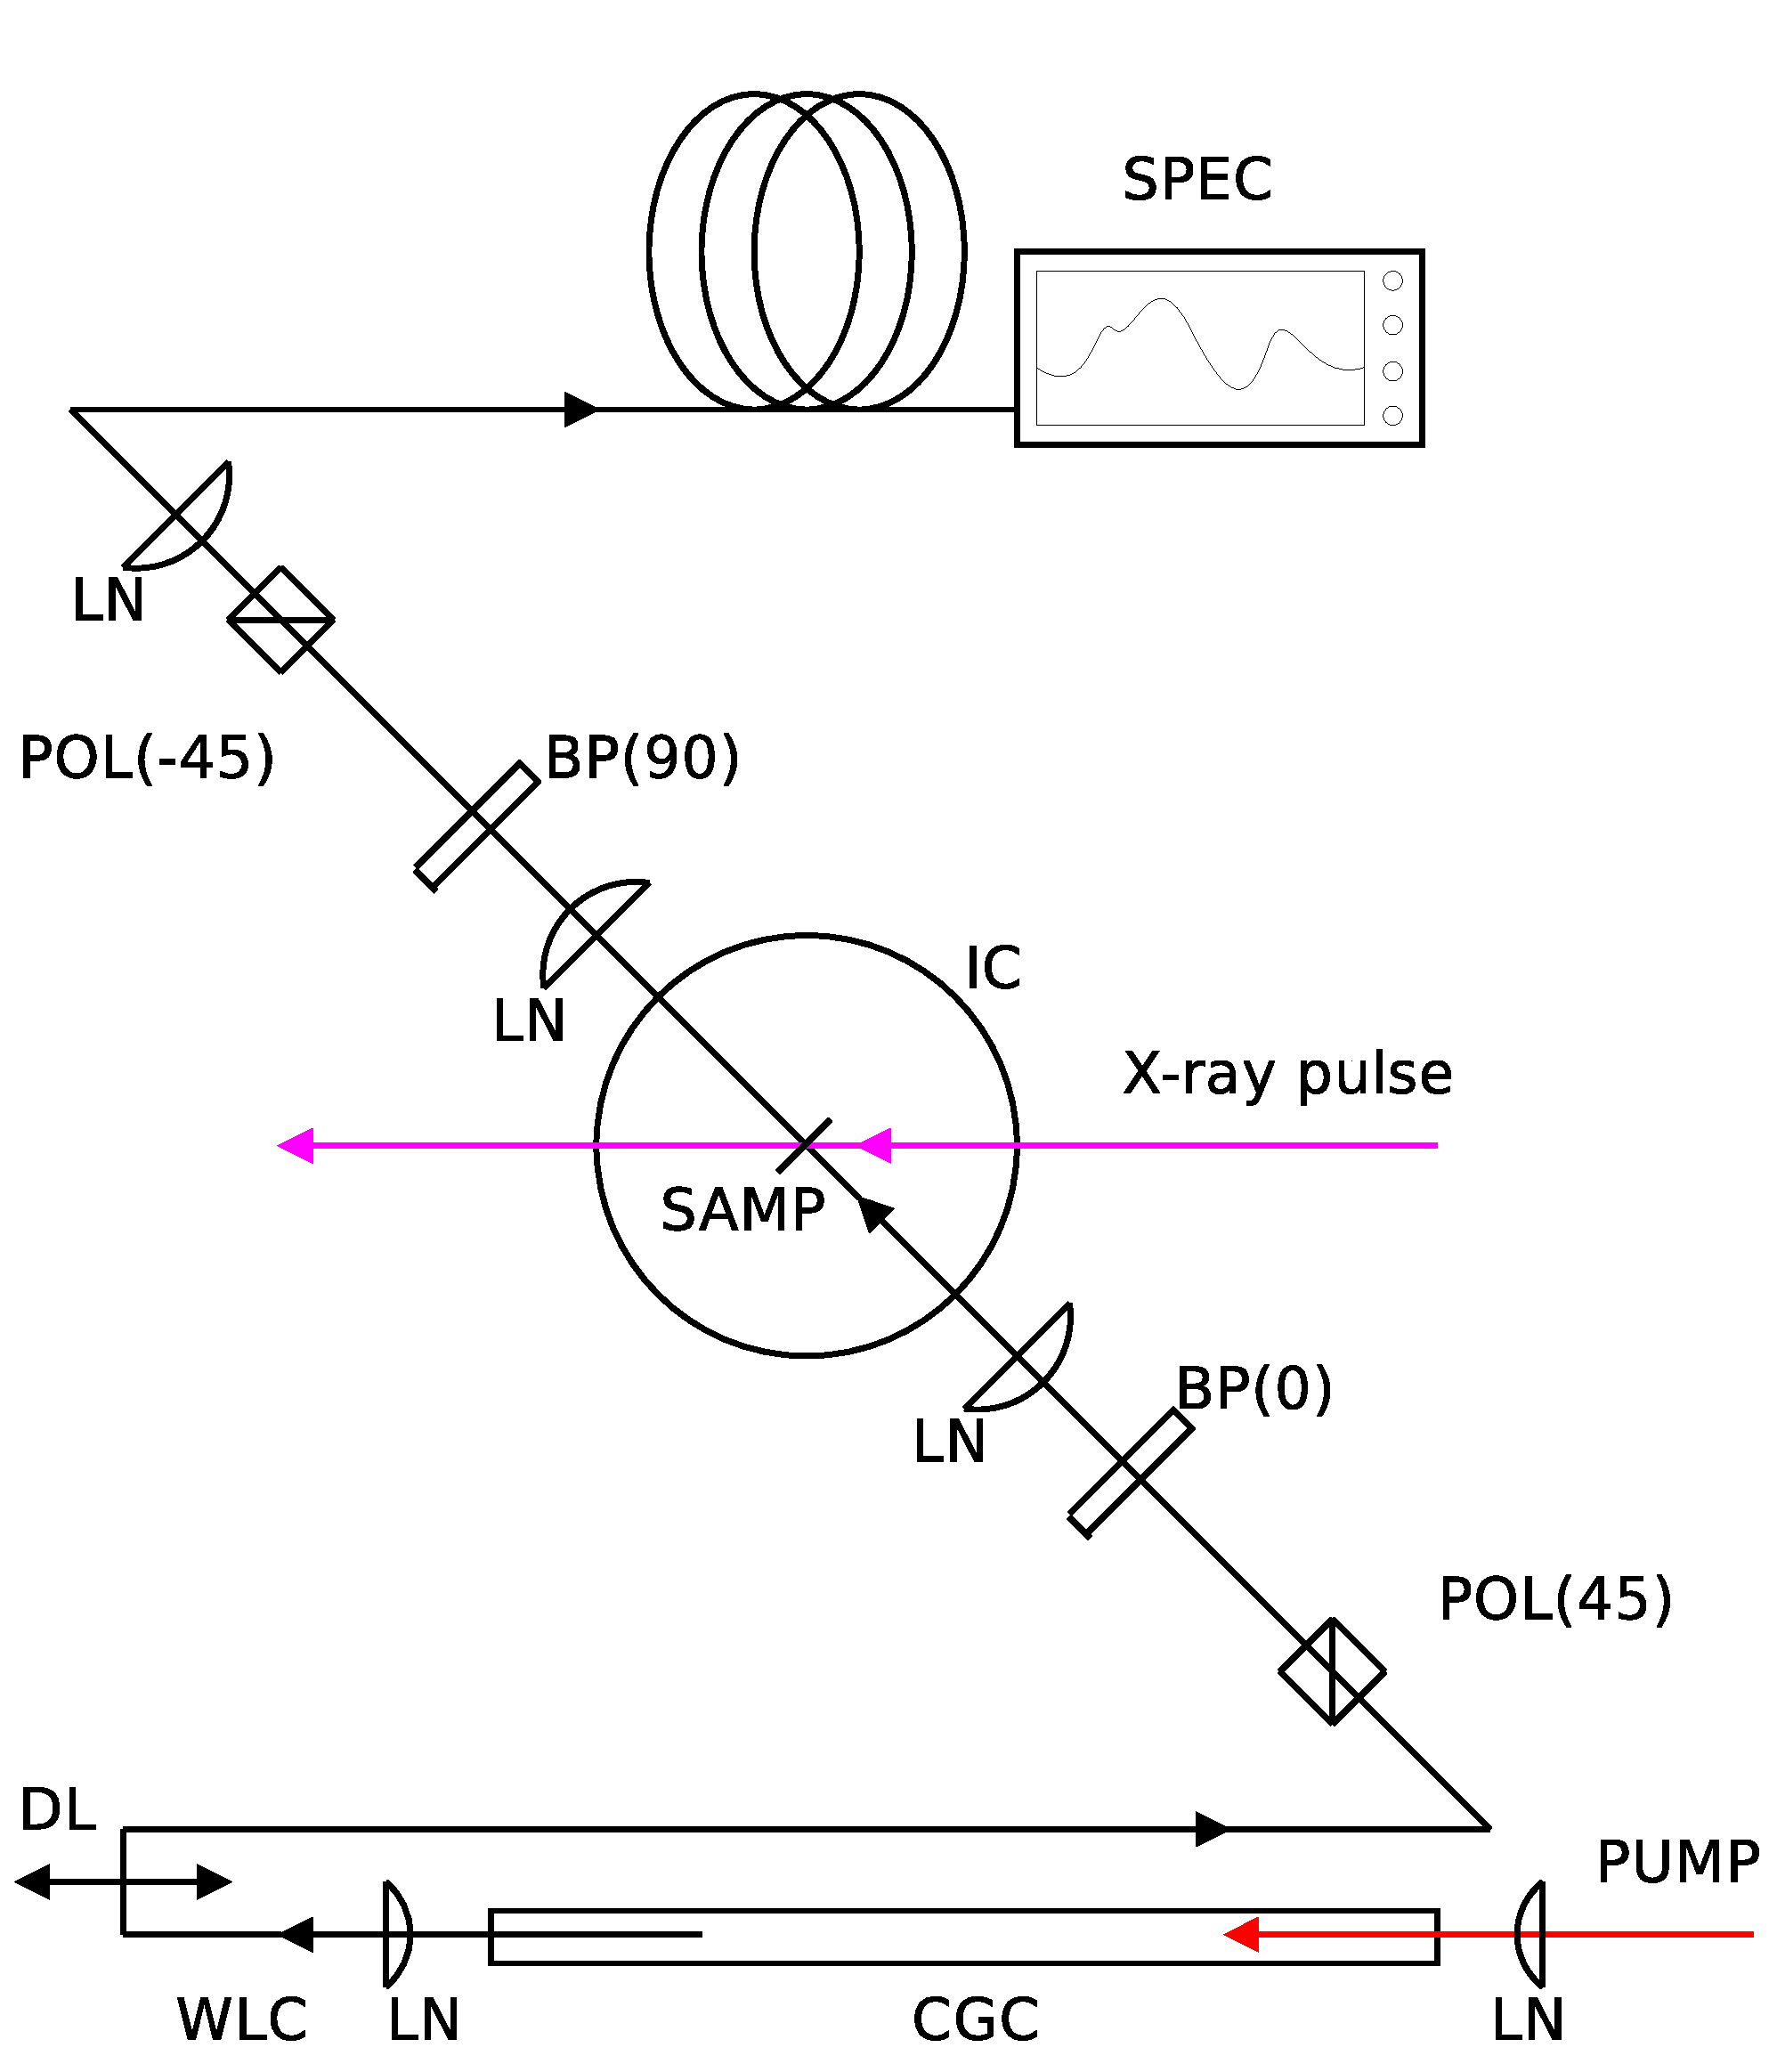
\includegraphics[width=.5\figwidth]{Scheme_diagram.eps}}
\caption{\label{fig::cartoon} Schmatic of the experimental design. 
PUMP -- 800 nm 50 fs pump laser pulse,
LN -- lens, 
CGC -- Continuum Gas Cell, 
WLC -- White Light Continuum, 
DL -- Delay Line, 
POL($x$) -- Polarizer (angle), 
BP($x$) -- Birefringent Plate (fast-axis alignment angle), 
SAMP -- Sample, 
X-ray pulse, 
IC -- interaction Chamber, 
SPEC -- Optical Spectrometer.
}
\end{figure}
\subsection{Whitelight Generation}
150 $\mu$J in 50 fs pulse to pump a cell of 200 PSI of Argon. 
\subsection{Birefringent delay}
\subsection{Substrates}
Diamond
Crossed polarization analysis

\section{Results}
\subsection{Phase not Absorption}
Signals in water and diamond
\subsection{X-ray Photon energy dependence}
\subsection{Optical wavelength dependence}

\section{Discussion}
\subsection{Material index change}
review a bit of the carrier dynamics that causes the index change
\subsection{algorithm}
\begin{figure}
\centerline{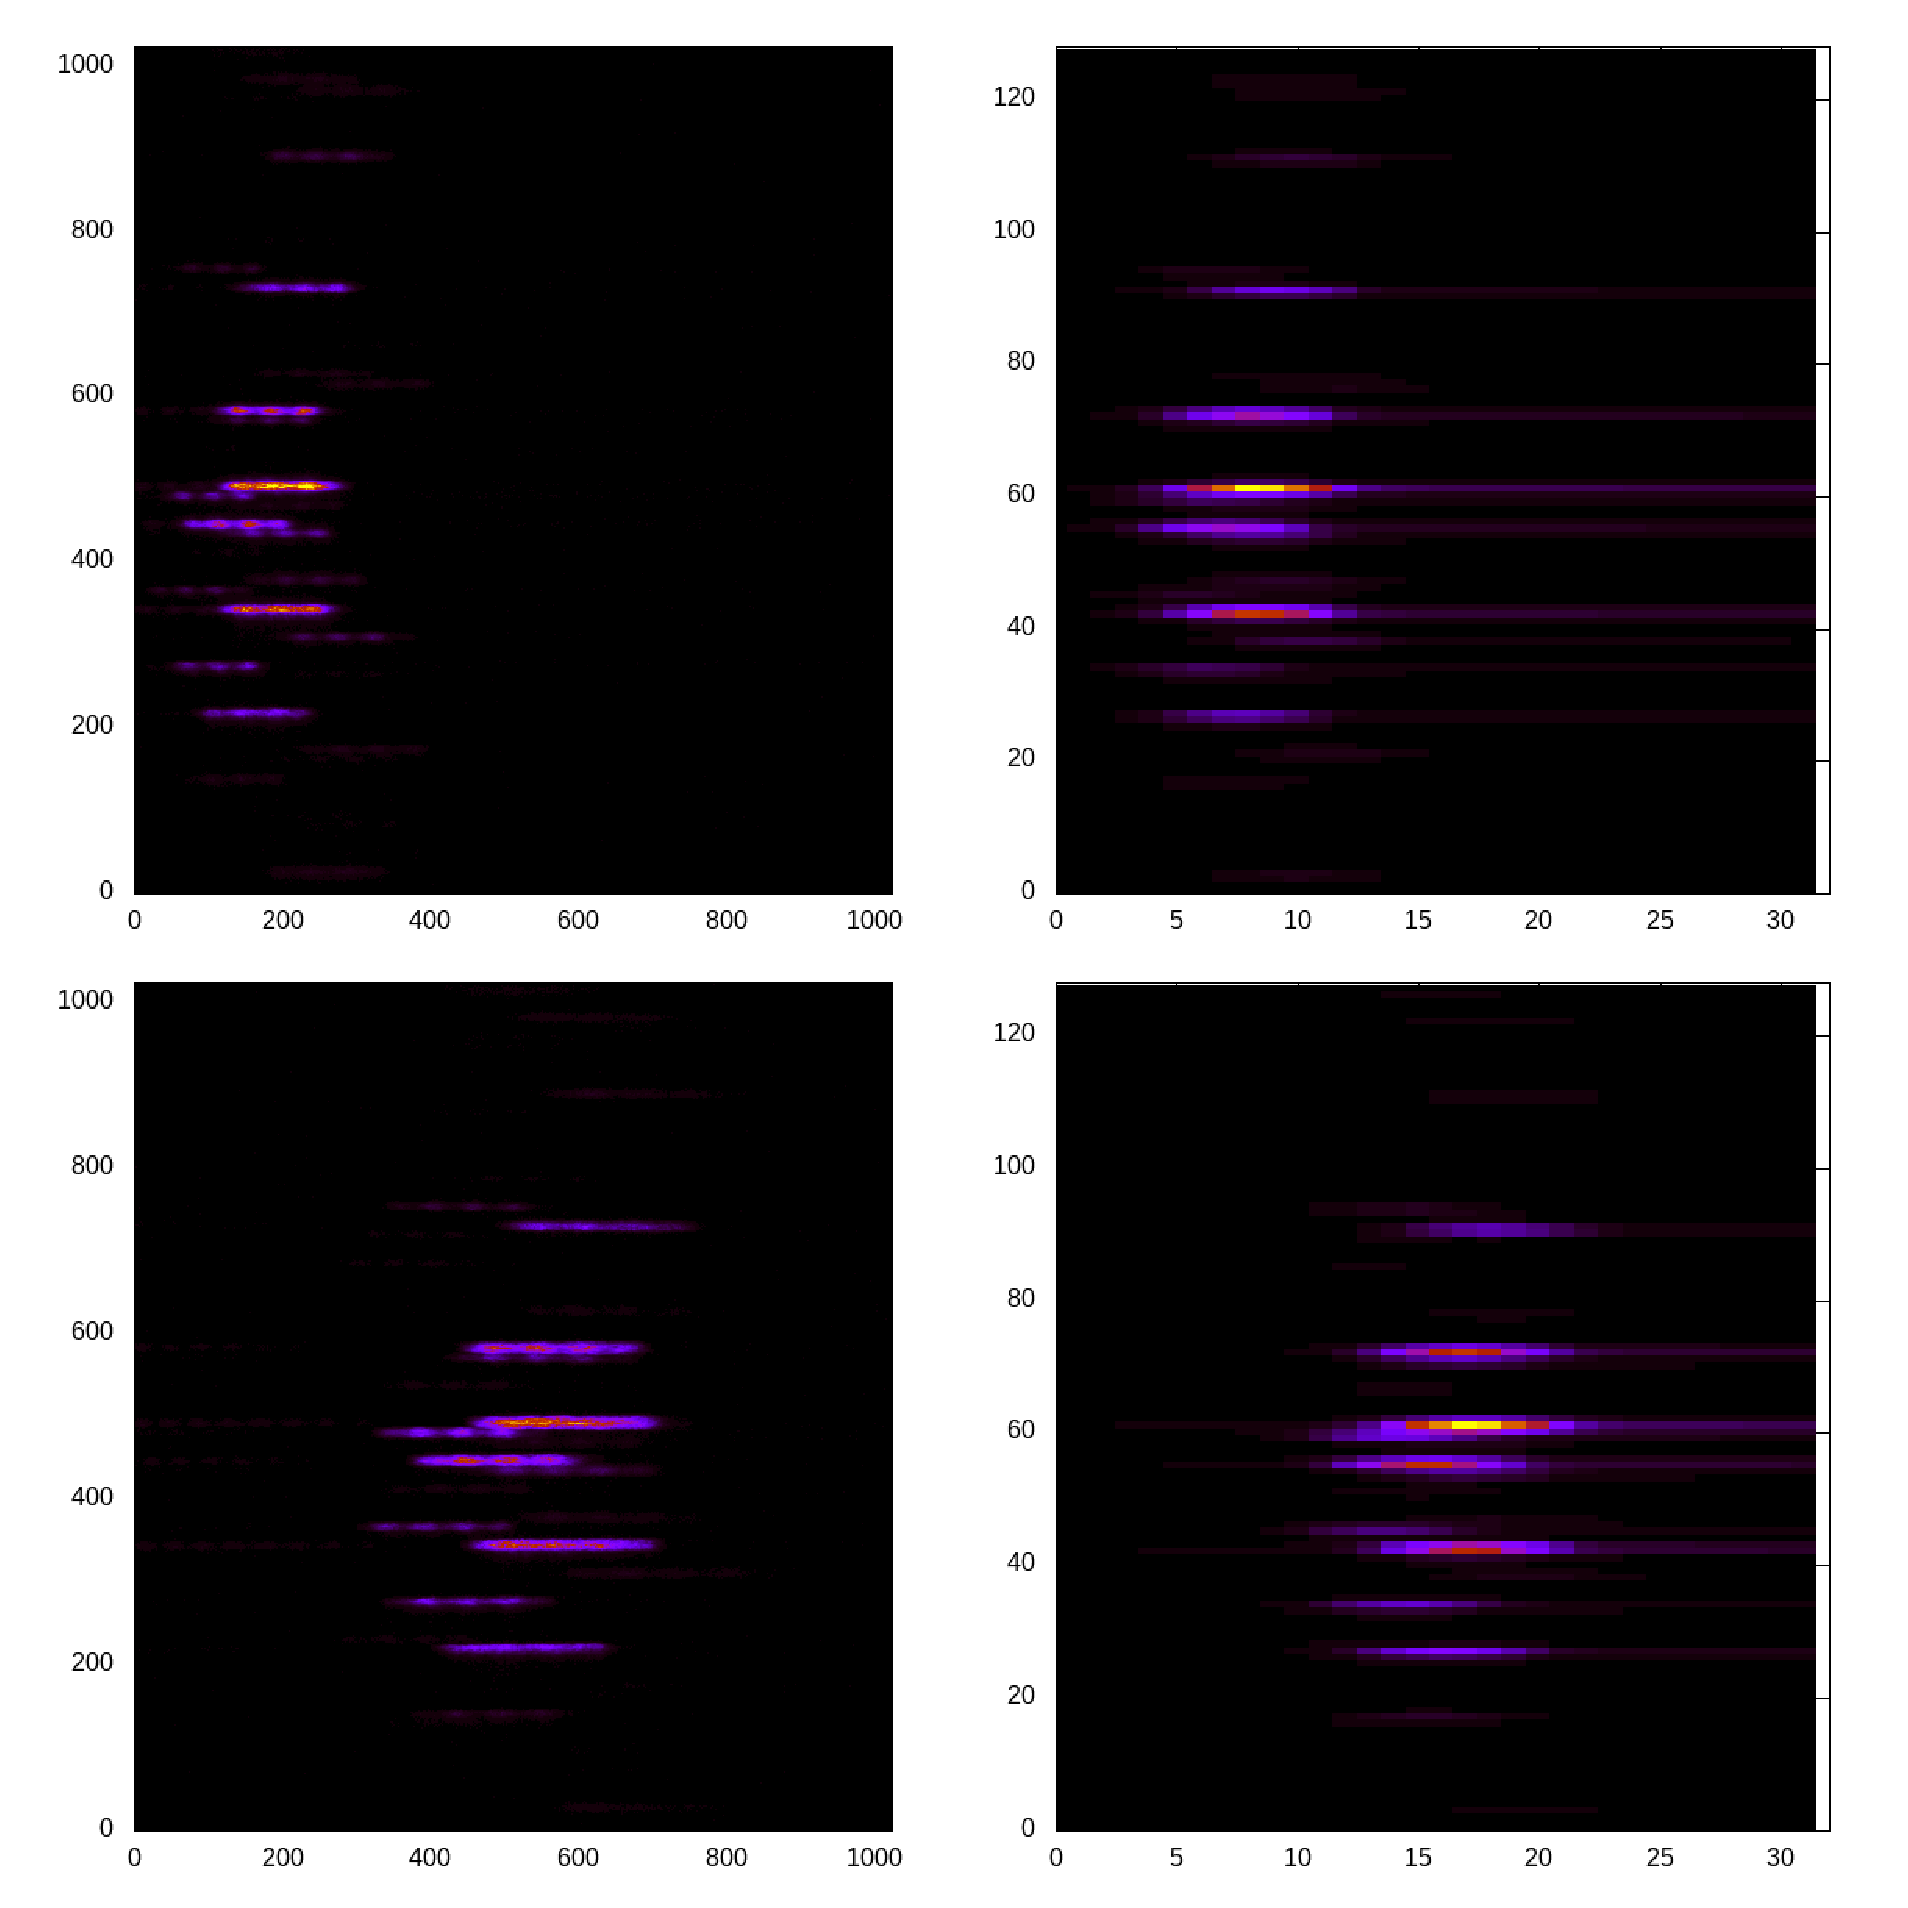
\includegraphics[width=.5\figwidth]{plotting.ip_method_exp.eps}}
\caption{\label{fig::ip_mthod}Use a non-2D version of this figure.}
\end{figure}
\subsection{Signal versus ev/atom (XPP/AMO)}

\subsection{Temporal Resolution (XPP)}
\subsection{Using the etalon (AMO)}

\section{Conclusion}

\bibliographystyle{plain}
\bibliography{$BIBFILES/Coffee,$BIBFILES/lcls_refs}
\end{document}


\end{document}

